\chapter{Defining the problem}

\section{Predict whether salary exceeds 50,000}
Prediction task is to determine whether a person makes over 50K a year by given data for his social background. 

\section{History of the dataset}
Extraction was done by Barry Becker from the 1994 Census database
The dataset has 48,882 instances, 14 attributes, has missing values and our problem is a class

\section{Attribute information}
The dataset contains the following attributes about a person ~\cite{uci-link}:
\begin{enumerate}
    \item Age - continuos
    \item Workclass - Private, Self-emp-not-inc, Self-emp-inc, Federal-gov, Local-gov, State-gov, Without-pay, Never-worked.
    \item Fnlwgt - sample weighting; this should be ignored while creating models
    \item Education - Bachelors, Some-college, 11th, HS-grad, Prof-school, Assoc-acdm, Assoc-voc, 9th, 7th-8th, 12th, Masters, 1st-4th, 10th, Doctorate, 5th-6th, Preschool. 
    \item Education-num: continuous (how many years has one learned)
    \item Marital status: Married-civ-spouse, Divorced, Never-married, Separated, Widowed, Married-spouse-absent, Married-AF-spouse. 
    \item Occupation: Tech-support, Craft-repair, Other-service, Sales, Exec-managerial, Prof-specialty, Handlers-cleaners, Machine-op-inspct, Adm-clerical, Farming-fishing, Transport-moving, Priv-house-serv, Protective-serv, Armed-Forces.
    \item Relationship: Wife, Own-child, Husband, Not-in-family, Other-relative, Unmarried. 
    \item Race: White, Asian-Pac-Islander, Amer-Indian-Eskimo, Other, Black. 
    \item Sex: Female, Male. 
    \item Capital gain: continuous, how much an individual has learned outside his usual wage
    \item Capital loss: continuous, how much an individual has lost outside his usual wage.
    \item Hours per week: continuous, how many hours per week an individual works
    \item Native country: United-States, Cambodia, England, Puerto-Rico, Canada, Germany, Outlying-US(Guam-USVI-etc), India, Japan, Greece, South, China, Cuba, Iran, Honduras, Philippines, Italy, Poland, Jamaica, Vietnam, Mexico, Portugal, Ireland, France, Dominican-Republic, Laos, Ecuador, Taiwan, Haiti, Columbia, Hungary, Guatemala, Nicaragua, Scotland, Thailand, Yugoslavia, El-Salvador, Trinadad and Tobago, Peru, Hong, Holand-Netherlands.
\end{enumerate}
\section{First look at the dataset}
There are a lot more examples from the first class (<50k earnings). If we always predict the majority class, we get accuracy of 76.07\%. This is a baseline accuracy, we obviously need result better than that. The accuracy metric is too biased and we will use the Kappa metric, since the classes are unbalanced. There are features of different scales. Two attributes have missing values: work class(6\%) and native country(2\%). There are no obvious correlation between the features and the output class \ref{fig:visual}.
\begin{figure}
    \centering
    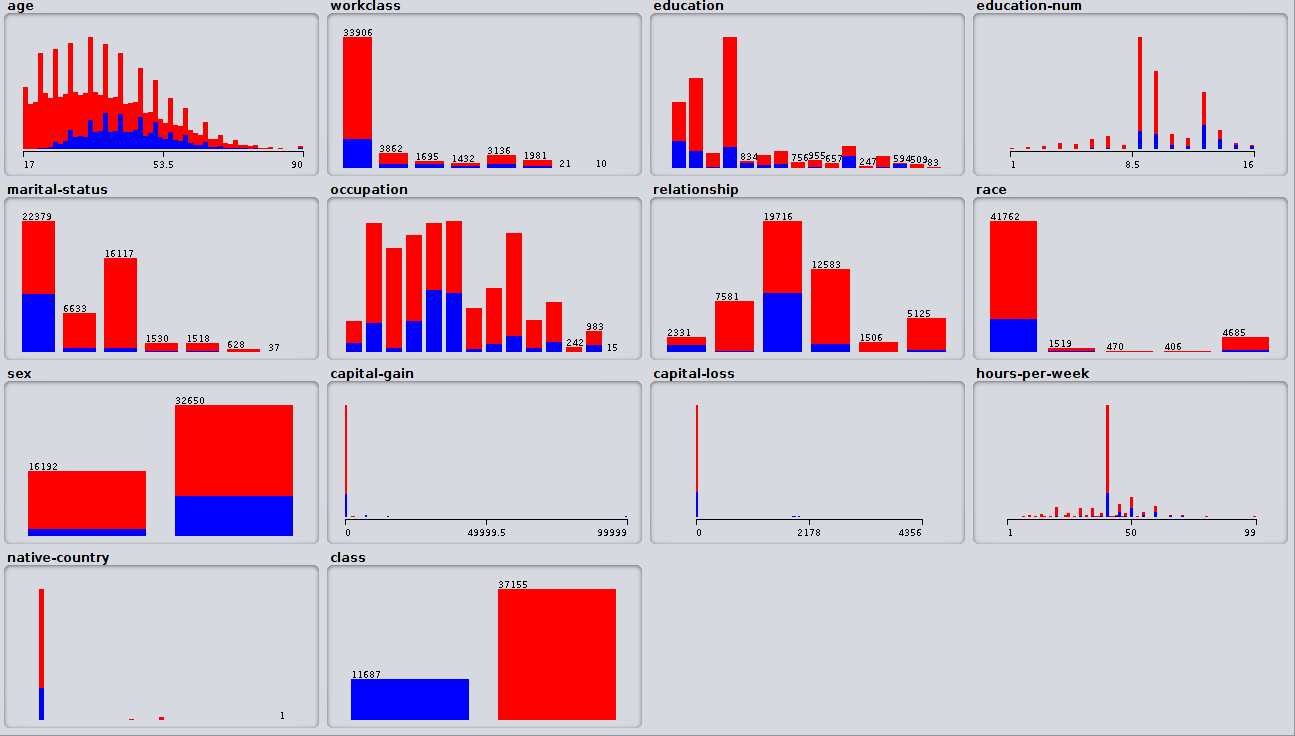
\includegraphics[scale=0.3]{visualize_all}
    \caption{Attributes correlation with output class visualized}
    \label{fig:visual}
\end{figure}

\chapter{Analyze the data}
\section{Handling missing values}
\section{Balancing classes}
\section{Normalization and standardization}
\section{Descriptive statistics}

\chapter{Prepare data}
\section{Raw view of the dataset}
\section{Normalized view of the dataset}
\section{Standardized view of the dataset}
\section{Dataset after feature selection}

\chapter{Evaluate algorithms}
\section{Initial experiment design}

\chapter{Impove results}
\section{Experiment for improving result}

\chapter{Present results}